\let\negmedspace\undefined
\let\negthickspace\undefined
\documentclass[journal]{IEEEtran}
\usepackage[a4paper, margin=10mm, onecolumn]{geometry}
%\usepackage{lmodern} % Ensure lmodern is loaded for pdflatex
\usepackage{tfrupee} % Include tfrupee package

\setlength{\headheight}{1cm} % Set the height of the header box
\setlength{\headsep}{0mm}  % Set the distance between the header box and the top of the text

\usepackage{gvv-book}
\usepackage{gvv}
\usepackage{cite}
\usepackage{amsmath,amssymb,amsfonts,amsthm}
\usepackage{algorithmic}
\usepackage{graphicx}
\usepackage{float}
\usepackage{textcomp}
\usepackage{xcolor}
\usepackage{txfonts}
\usepackage{listings}
\usepackage{enumitem}
\usepackage{mathtools}
\usepackage{gensymb}
\usepackage{comment}
\usepackage[breaklinks=true]{hyperref}
\usepackage{tkz-euclide} 
\usepackage{listings}
% \usepackage{gvv}                                        
\def\inputGnumericTable{}                                 
\usepackage[latin1]{inputenc}                                
\usepackage{color}                                            
\usepackage{array}                                            
\usepackage{longtable}                                       
\usepackage{calc}                                             
\usepackage{multirow}    
\usepackage{multicol}
\usepackage{hhline}                                           
\usepackage{ifthen}                                           
\usepackage{lscape}
\usepackage{tikz}
\usetikzlibrary{patterns}
\begin{document}


\title{GATE-01}
\author{ee25btech11063 - VEJITH}
\maketitle
% \maketitle
% \newpage
% \bigskip




\begin{enumerate}
\item Earth's dipole field originates mainly from

\hfill (GATE GG 2010)
\begin{multicols}{4}
\begin{enumerate}
\item mantle
\item outer core
\item inner core
\item crust
\end{enumerate}
\end{multicols}

\item  sunspots are regions of

\hfill (GATE GG 2010) 
\begin{multicols}{2}

\begin{enumerate}
\item high pressure
\item low magnetic field
\item high temperature
\item high magnetic field
\end{enumerate}
\end{multicols}

\item  The electrical conduction mechanism in  sedimentary rocks is usually.

\hfill (GATE GG 2010) 
\begin{multicols}{4}

\begin{enumerate}
\item pyroelectric
\item electronic
\item electrolytic
\item dielectric
\end{enumerate}
\end{multicols}


\item  The unit of electrical resistivity is

\hfill (GATE GG 2010) 
\begin{multicols}{4}

\begin{enumerate}
\item ohm
\item ohm-m
\item ohm-m$^2$
\item ohm-m$^{-1}$
\end{enumerate}
\end{multicols}

\item  outcrop pattern parallel to topographic contours signifies

\hfill (GATE GG 2010) 
\begin{multicols}{2}

\begin{enumerate}
    \item horizontal beds
    \item vertical beds
    \item inclined beds
    \item folded beds
\end{enumerate}
\end{multicols}

\item A rock with equal modal contents of quartz,plagioclase and orthoclase is known as

\hfill (GATE GG 2010)
\begin{multicols}{4}

\begin{enumerate}

\item diorite
\item gabbro
\item granite
\item syenite

\end{enumerate}
\end{multicols}


\item   The main factors in soil-forming processes are

\hfill (GATE GG 2010) 

\begin{enumerate}
\item bedrock and time only
\item topography and bedrock only
\item climate,time and topography only
\item climate,topography,bedrock and time
\end{enumerate}


\item  Glacial drift refers to the

\hfill (GATE GG 2010)

\begin{enumerate}
\item movement of glaciers
\item interglacial intervals
\item erosional landforms produced by glaciers
\item sediments deposited by glaciers
\end{enumerate}


\item  sand dunes are long ridges whose alignment is

\hfill (GATE GG 2010)

\begin{enumerate}
\item always parallel to prevailing wind direction
\item always perpendicular to prevailing wind direction
\item either parallel or perpendicular to prevailing wind direction
\item not related  to prevailing wind direction
\end{enumerate}


\item  The oldest rocks in India are

\hfill (GATE GG 2010)

\begin{enumerate}
\item more than $3$ billion years old
\item between $2.5$ and $3$ billion years old
\item between $2$ and $2.5$ billion years old
\item less than $2$ billion years old
\end{enumerate}


\item  The sequential placement of geological events as determined by their position in the rock record is known as

\hfill (GATE GG 2010) 
\begin{multicols}{2}

\begin{enumerate}
\item relative dating
\item correlation
\item absolute dating
\item uniformitarianism
\end{enumerate}
\end{multicols}

\item  Time equivalence of rock units in different areas  can be established primarily by considering similarity in

\hfill (GATE GG 2010)
\begin{multicols}{4}

\begin{enumerate}
\item lithology
\item fossil assemblages
\item sedimentary structures
\item mineral assemblages
\end{enumerate}
\end{multicols}


\item  Which of the following volcanic events has been suggested as a major cause of the extinction of dinosaurs?

\hfill (GATE GG 2010) 
\begin{multicols}{2}

\begin{enumerate}
\item Panjal volcanism
\item Deccan volcanism
\item Rajmahal volcanism
\item Malani volcanism
\end{enumerate}
\end{multicols}

\item Bode's law express the approximate distance between

\hfill (GATE GG 2010) 

\begin{enumerate}
\item earth and other planets
\item moon and sun
\item planets and sun
\item moon and earth
\end{enumerate}

\item  India's northward drift from Gondwanaland is believed to have started approximately (in million years ago,Ma) 

\hspace*{15.7cm}(GATE GG 2010)
\begin{multicols}{4}
\begin{enumerate}
\item $50$ Ma
\item $150$ Ma
\item $300$ Ma
\item $400$ Ma
\end{enumerate}
\end{multicols}

\item  Which of the following instruments contain piezoelectric material?

\hfill (GATE GG 2010)
\begin{multicols}{2}

\begin{enumerate}
\item hydrophone
\item geophone
\item gravimeter
\item magnetometer
\end{enumerate}
\end{multicols}


\item  If the average crustal thickness is $35$ km and the height of a mountain is $5$ km above the mean sea level.the crustal thickness on Airy's  model beneath the mountain will be approximately

\hfill (GATE GG 2010)
\begin{multicols}{4}

\begin{enumerate}

\item $35$ km
\item $40$ km
\item $50$ km
\item $70$ km
\end{enumerate}
\end{multicols}

\item The equipotential surface over which the gravitational field has equal value is known as 

\hfill (GATE GG 2010) 
\begin{multicols}{2}

\begin{enumerate}
\item geoid
\item spheroid
\item ellipsoid
\item mean sea level
\end{enumerate} 
\end{multicols}

\item The angle between the present geographic north and geomagnetic north is

\hfill (GATE GG 2010) 
\begin{multicols}{4}

\begin{enumerate}
\item$1.5\degree$
\item$7.5\degree$
\item$11.5\degree$
\item$23.5\degree$
\end{enumerate}
\end{multicols}

\item Among the following the best reconnaissance method for determining basement configuration of sedimentary basins is\\

\hfill(GATE GG 2010)
\begin{multicols}{2}
\begin{enumerate}
    \item gravity method
    \item self potential method
    \item seismic method
    \item electromagnetic method
\end{enumerate}
\end{multicols}

\item Cooling of basic lava under water will lead to the formation of

\hfill (GATE GG 2010)
\begin{multicols}{2}

\begin{enumerate}
    \item lava tunnel
    \item pillow structure
    \item columnar jointing
    \item cumulus texture
\end{enumerate}
\end{multicols}

\item What would you expect to find at the base of a typical oceanic plate?

\hfill (GATE GG 2010) 
\begin{multicols}{4}

\begin{enumerate}
    \item Basalt
    \item Diorite
    \item Gabbro
    \item peridotite
\end{enumerate}
\end{multicols}

\item Major coal deposits of India are found in the

\hfill (GATE GG 2010)
\begin{multicols}{2}

\begin{enumerate}
    \item cuddapah supergroup
    \item vindhyan supergroup
    \item Gondwana supergroup
    \item Dharwar supergroup
\end{enumerate}
\end{multicols}

\item Which of the following is a product of residual weathering process?

\hfill (GATE GG 2010)
\begin{enumerate}
\begin{multicols}{2}
    \item Placer gold
    \item Banded iron ore
    \item Bauxite
    \item Porphyry copper
\end{multicols}
\end{enumerate}

\item Choose the correct combination of ore and location of it's deposits.

\hfill (GATE GG 2010)



\begin{enumerate}
\begin{multicols}{2}
    \item uranium-jaduguda
    \item Lead-khetri
    \item Gold-panna
    \item Iron-Malanjkhand
\end{multicols}
\end{enumerate}

\item The age of the oldest rocks in present-day ocean basins is

\hfill (GATE GG 2010) 
\begin{multicols}{4}

\begin{enumerate}
    \item Devonian
    \item Jurassic
    \item Eocene
    \item Permian
\end{enumerate}
\end{multicols}
\item Silicon to oxygen ratio in the following silicate structure is

\hfill (GATE GG 2010) 
\begin{multicols}{4}

\begin{figure}[H]
    \centering
    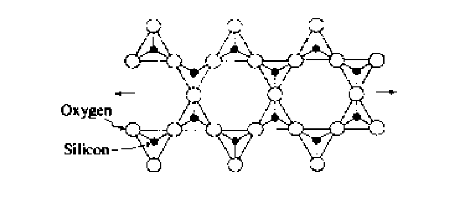
\includegraphics[width=0.5\linewidth]{figs/01.png}
    \caption{silicate structure}
    \label{fig:silicate}
\end{figure}
\begin{enumerate}
    \item $1:2$
    \item $2:5$
    \item $4:11$
    \item $1:3$
\end{enumerate}
\end{multicols}

\item Direct precipitation of uraninite from a mineralizing solution containing  $UO_2$ions can take place due to

\hfill (GATE GG 2010) 
\begin{multicols}{2}

\begin{enumerate}
    \item increase in Eh
    \item decrease in Eh
    \item increase in pH
    \item  decrease in pH
\end{enumerate}
\end{multicols}

\item Match the optical properties  in Group I with appropriate minerals in Group II.

\hfill (GATE GG 2010) \\
\begin{tabular}{ l l }
\textbf{Group I} & \textbf{Group Il}\\

P. Twinkling & 1. Quartz\\
Q. Pleochroic haloes & 2. Nepheline\\
R. Anomalous interference colour & 3. Calcite\\
S. Uniaxial positive & 4. Chloride\\
	& 5.Biotite \\
\end{tabular}
\begin{multicols}{2}
\begin{enumerate}

    \item P$- 4$, Q$- 5$, R$- 3$, S$- 2$
    \item P$- 3$, Q$- 4$, R$- 5$, S$- 2$
    \item P$- 3$, Q$- 5$, R$- 4$, S$- 1$
    \item P$- 3$, Q$- 4$, R$- 5$, S$- 1$
\end{enumerate}
\end{multicols}

\item Wall-rock alteration producing epidote, albite and chloride around an ore body is called 

\hfill (GATE GG 2010) 
\begin{multicols}{2}

\begin{enumerate}
    \item argillic alteration
    \item propylitic alteration
    \item potassium-silicate alteration
    \item sericite alteration
\end{enumerate}
\end{multicols}
\item Match the textures/structures  in Group I with appropriate minerals in Group II.

\hfill (GATE GG 2010) \\

\begin{tabular}{ l l }
\textbf{Group I} & \textbf{Group Il}\\

P.Cumulus texture & 1. Cavity filling\\
Q.Spinifex texture & 2. Gravity settling\\
R.Oriented intergrowth & 3. Annealing\\
S.Comb structure & 4. Quenching\\
& 5. Coherent exsolution \\
\end{tabular}
\begin{multicols}{2}
\begin{enumerate}
    \item  P$- 2$, Q$- 4$, R$- 5$, S$- 1$
     \item P$- 3$, Q$- 1$, R$- 2$, S$- 5$
      \item P$- 1$, Q$- 5$, R$- 4$, S$- 3$
       \item P$- 2$, Q$- 5$, R$- 4$, S$- 1$ 
\end{enumerate}

\end{multicols}

\item An area shows linear erosional depression, sag pond, spring and offset stream along with sub-horizontal slickensides. The prominent structure indicated by these features is

\hfill (GATE GG 2010)
\begin{multicols}{2}

\begin{enumerate}
    \item strike-slip fault
    \item horst and graben
    \item klippe
    \item nappe
\end{enumerate}
\end{multicols}

\item  Match the ore types  in Group I with path-finder elements in Group Il

(GATE GG 2010)\\
\begin{tabular}{ l l }
\textbf{Group I} & \textbf{Group Il}\\

P. Porphyry Cu ore & 1.As\\
Q. Vein type Au ore & 2.Hg\\ 
R. Pb-Zn-Ag ores & 3.Cr\\
& 4.Mo\\
& 5.Ni\\
\end{tabular}
\begin{multicols}{2}
\begin{enumerate}

\item P$- 4$, Q$- 1$, R$- 2$
\item P$- 3$, Q$- 2$, R$- 1$
\item P$- 4$, Q$- 3$, R$- 5$
\item P$- 5$, Q$- 4$, R$- 2$
\end{enumerate}
\end{multicols}


\item Match the nature of mass movements listed in Group I with the evidences listed in Group II.

\hfill (GATE GG 2010) \\
\begin{tabular}{ l l }
\textbf{Group I} & \textbf{Group Il}\\



P. Creep & 1.Tounge-shaped mass movement\\
Q. Earth flow & 2. Curved tree trunks\\
R. Slump & 3. Scree formation at the base\\
& 4. Curved surface of rupture
\end{tabular}
\begin{multicols}{2}
\begin{enumerate}

    \item P$- 2$, Q$- 1$, R$- 4$
    \item P$- 1$, Q$- 3$, R$- 4$
    \item P$- 4$, Q$- 2$, R$- 1$
    \item P$- 4$, Q$- 3$, R$- 2$
\end{enumerate}
\end{multicols}

\item Which of the following metamorphic facies is characterized by the pyrope rich garnet$+$ omphacite assemblage?

\hfill (GATE GG 2010) 
\begin{multicols}{2}

\begin{enumerate}

     \item Blueschist
     \item Eclogite
     \item Greenschist
     \item Granulite

\end{enumerate}
\end{multicols}
\item Match the gemstones in Group I with corresponding minerals in Group II.

\hfill (GATE GG 2010) \\
\begin{tabular}{ l l }
\textbf{Group I} & \textbf{Group Il}\\
P. Peridote & 1. Beryl\\
Q. Emerald & 2. Feldspar\\
R. Amazonite & 3. Corundum\\
S. Ruby & 4. Olivine\\
\end{tabular}
\begin{multicols}{2}
\begin{enumerate}

    \item  P$- 4$, Q$- 1$, R$- 2$, S$- 3$
    \item  P$- 1$, Q$- 3$, R$- 2$, S$- 4$
    \item  P$- 2$, Q$- 4$, R$- 1$, S$- 3$
    \item  P$- 3$, Q$- 4$, R$- 1$, S$- 2$
\end{enumerate}
\end{multicols}

\item Which of the following statements is NOT correct with regard to a perched water table?

\hfill (GATE GG 2010) 

\begin{enumerate}

    \item It is within an area where a local aquiclude occurs within a larger aquifer
    \item It lies above the main water table
    \item It is found in the main zone of saturation
    \item It is occasionally associated with springs

\end{enumerate}
\item The spatial resolution of IRS LISS-III multi-spectral sensor for Near Infra-Red (NIR) band is

\hfill (GATE GG 2010) 
\begin{multicols}{4}

\begin{enumerate}
    \item $5.8\text{m}\times 5.8\text{m}$ 
    \item $23.5\text{m}\times 23.5\text{m}$
    \item $70\text{m}\times 70\text{m}$
    \item $72.5\text{m}\times 72.5\text{m}$ 
\end{enumerate}
\end{multicols}

\item Which of the following combinations of extinction events and extinct organisms is NOT correct?

\hfill (GATE GG 2010) 
\begin{multicols}{2}

\begin{enumerate}
    \item Cretaceous end Dinosaurs
    \item Triassic end-Conodonts
    \item Permian end - Trilobites
    \item Miocene end - Ammonites
\end{enumerate}
\end{multicols}

\item In India, marine fossili ferous rocks of lower Paleozoic age are mainly found in the

\hfill (GATE GG 2010)

\begin{enumerate}
\begin{multicols}{2}
    \item Gondwana
    \item Higher Himalaya
    \item Outer Himalaya
    \item Tethys Himalaya
\end{multicols}
\end{enumerate}

\item Which of the following pairs of rock formations and characteristic fossils is correct?

\hfill (GATE GG 2010)
\begin{multicols}{2}

\begin{enumerate}
    \item Raniganj-$Elephas$
    \item Pinjor-$Titanosaurus$
    \item Lameta-$Glossopteris$
    \item Subathu-$Nummulites$
\end{enumerate}
\end{multicols}

\item Which of the following groups of rock formations is NOT arranged from older to younger?

\hfill (GATE GG 2010) 

\begin{enumerate}
    \item Uttatur Trichinopoly Ariyalur - Niniyur
    \item Paicham-Katrol-Chari - Urmia
    \item Talchir-Damuda Panchet - Mahadev
    \item Semri-Kaimur-Rewa-Bhander
\end{enumerate}

\item Choose the correct combination of geological agents and associated features

\hfill (GATE GG 2010) 
\begin{multicols}{2}

\begin{enumerate}
    \item River - Spit
    \item Glacier Yardang
    \item Longshore current - Esker
    \item Wind-Ventifact
\end{enumerate}
\end{multicols}

\item A sedimentary sequence dominated by large scale (5-10 m thick) cross beds, well-sorted and well-rounded quartz-rich sand with no fine matrix is most likely to be a

\hfill (GATE GG 2010) 

\begin{enumerate}
    \item deltaic deposit
    \item lagoonal deposit
    \item colian deposit
    \item outer shelf deposit
\end{enumerate}

\item An invertebrate in which the plane of symmetry bisects the shell through the mid-point of the hinge is a

\hfill (GATE GG 2010) 
\begin{multicols}{4}

\begin{enumerate}
    \item Pelecypod
    \item Brachiopod
    \item Gastropod
    \item Caphalopod
\end{enumerate}
\end{multicols}

\item The oldest mamals and birds are known ,respectively from,

\hfill (GATE GG 2010) 

 \begin{enumerate}
 \item Creataceous and paleocene
  \item Silurian and Devonian
   \item Triassic and Jurassic
    \item Oligocene and Miocene
 
\end{enumerate}


\item Allochems in a limestone consist of

\hfill (GATE GG 2010)

\begin{enumerate}
    \item micrite only
    \item spar only
    \item ooids only
    \item bioclasts and ooids
\end{enumerate}

\textbf{Common Data Questions}\\

\textbf{Common Data Questions 48 and 49}

 The following geological map exposes three beds, of which the bed P is the oldest and the bed R the youngest.
 
\hfill(GATE GG 2010)

\begin{figure}[H]
    \centering
    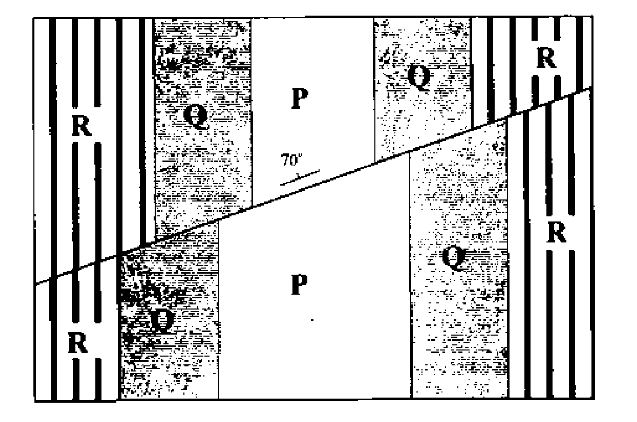
\includegraphics[width=0.5\linewidth]{figs/02.png}
    \caption{}
    \label{fig:2}
\end{figure}
\item What type of structure does the map depict?

\hfill (GATE GG 2010) 
\begin{multicols}{2}

\begin{enumerate}
    \item Faulted anticline
    \item Folded strike-slip fault
    \item Faulted syncline
    \item Folded normal fault
\end{enumerate}
\end{multicols}

\item Why is bed P wider in the area south of fault?

\hfill (GATE GG 2010) 

\begin{enumerate}
    \item Erosion has removed most of bed P to the north of fault
    \item Folding has caused thinning of bed P to the north of fault
    \item Deeper level of bed P is exposed due to faulting and erosion to the south of fault
    \item Bed P had a variable thickness prior to faulting
\end{enumerate}

\textbf{Common Data Questions 50 and 51}\\
A sequence of shale and limestone is intruded by an igneous pluton. Metasomatic interaction between the pluton and the country rocks involves introduction of Si and Al isto dolomitic limestone.

\item  Which pair of rock types best describes the products of metamorphism in the contact aureole?

\hfill(GATE GG 2025)
\begin{multicols}{2}
\begin{enumerate}

    \item Slate and schist
    \item Schist and skarn
\item Schist and bornfels
\item Hornfels and skarn
\end{enumerate}
\end{multicols}

\item The mineral which is NOT expected in assemblages in the metamorphosed dolomitic limestone is

\hfill (GATE GG 2010) 
\begin{multicols}{2}

\begin{enumerate}
    \item coarse
    \item  anorthite
\item diopside
\item andalusite
\end{enumerate}
\end{multicols}

\textbf{Linked Answer Questions}\\
\textbf{statement for Linked Answer Questions 52 and 53:}

A pluton of iron-poor basic magma containing trace concentrations of Ni, Rb, Sr and V undergoes crystallization upon cooling
\item The first mineral to crystallize will be

\hfill (GATE GG 2010) 
\begin{multicols}{4}

\begin{enumerate}
    \item augite

 \item hornblende

 \item olivine

 \item oligoclase

\end{enumerate}
\end{multicols}

\item The trace element that will be preferentially incorporated in the correct mineral in Q. 52 is

\hfill (GATE GG 2010) 
\begin{multicols}{4}

\begin{enumerate}
    \item Ni

\item Rb

\item Sr

\item V
\end{enumerate}
\end{multicols}

\textbf{Linked Answer Questions 54 and 55:}
\item Silica-undersaturated minerals are

\hfill (GATE GG 2010) 
\begin{multicols}{2}

\begin{enumerate}
    \item nepheline and albite

\item  olivine and enstatite

\item leucite and orthoclase

\item olivine and leucite

\end{enumerate}
 \end{multicols}
 
\item The Hermann-Mauguin symbols of crystallographic notation for the correct minerals in Q. 54 are

\hfill (GATE GG 2010) 
\begin{multicols}{2}

\begin{enumerate}
    \item $2/ \text{m}2/ \text{m}2/ \text{m}$ and $4/ \text{m}$
    \item $2/ \text{m}2/ \text{m}2/ \text{m}$ for both
    \item $4/ \text{m}$ and  $2/ \text{m}$
    \item $6$ and I
    
\end{enumerate}
\end{multicols}
\end{enumerate}
\textbf{END OF SECTION 1 OF PART B}



\textbf{PART B (SECTION 2): FOR GEOPHYSICS CANDIDATES ONLY}
\begin{enumerate}[start=26]
    \item The gravity value measured at the base of a 10 m tall building is 40 mGal. The value at the top of the building ignoring its mass is close to
    
\hfill (GATE GG 2010) 
\begin{multicols}{4}

\begin{enumerate}
    \item $20$ mGal
\item  $37$ mGal
\item $40$ mGal
\item $43$ mGal
\end{enumerate}
\end{multicols}

\item Upward continuation technique filters their wavelength anomalies and amplitudes.

\hfill (GATE GG 2010) 
\begin{enumerate}
    \item short. reduces

\item long, enhances

\item long, reduces
\item  short, enhances
\end{enumerate}

\item The relative intensities of induced and remanent magnetization are 

commonly expressed in terms of

\hfill (GATE GG 2010) 
\begin{enumerate}
    \item  susceptibility

\item  gyromagnetic ratio

\item  Poisson's ratio

\item konigsberg ratio
 
\end{enumerate}
\item  In electrical resistivity method, which among the following is correct with reference to Geometric Factor(GF)? 

\hfill(GATE GG 2010)

\begin{enumerate}

     \item  varies for profiling and remains constant for sounding

\item  GF remains constant for both profiling and sounding

\item GF remains constant for profiling and varies for sounding

\item GF varies for both profiling and sounding

\end{enumerate}

\item If in a magnetic dipole $'m'$ represents poles of equal strength and $'l'$ represents the distance between the two poles, then the magnetic moment of dipole is

\hfill (GATE GG 2010) 
\begin{multicols}{4}

\begin{enumerate}
    \item $lm$
    \item $\frac{l}{m}$
    \item $2lm$
    \item $\frac{lm}{2}$
\end{enumerate}
\end{multicols}

\item  Energy in radioactive decay with respect to time follows

\hfill (GATE GG 2010) 

\begin{enumerate}
    \item normal distribution
\item Poisson distribution
\item chi-squared distribution
\item binomial distribution
\end{enumerate}

\item The logging technique that uses non-conductive drilling fluids is

\hfill (GATE GG 2010) 
\begin{enumerate}
 \item  SP logging
\item  Resistivity logging
\item Induction logging
\item Radiometric logging
\end{enumerate}

\item Unguided random-walk inversion technique signifies

\hfill (GATE GG 2010) 
\begin{enumerate}
 \item  Genetic algorithm
\item Simulated annealing
\item Monte Carlo inversion
\item Metropolis algorithm
\end{enumerate}
\item The compressional wave velocity V$p$ within a solid with adiabatic bulk modulus K$\gamma$ rigidity modulus G and density $\rho$ is given by

\hfill (GATE GG 2010) 
\begin{multicols}{2}

\begin{enumerate}
\item v$p=\sqrt{\frac{k\gamma +(5/3)G}{\rho}}$
\item v$p=\sqrt{\frac{k\gamma +(2/3)G}{\rho}}$
\item v$p=\sqrt{\frac{k\gamma +(1/3)G}{\rho}}$
\item v$p=\sqrt{\frac{k\gamma +(4/3)G}{\rho}}$
\end{enumerate}
\end{multicols}

\item The number of independent elements of the $4th$ order stiffness tensor required to characterize general elastic media is 

\hfill(GATE GG 2010)
\begin{multicols}{4}
\begin{enumerate}
    \item  2
    \item 21
    \item 36
    \item 81 
\end{enumerate}
\end{multicols}

\item The seismic energy released in an earthquake of magnitude M$s$ = 7.0 is about $\hrulefill$  times that released in an earthquake of M$s$ = 6.0. times that

\hfill (GATE GG 2010) 
\begin{multicols}{4}

\begin{enumerate}
    \item  10

\item  32

\item 64

\item 100
\end{enumerate}
\end{multicols}

\item In the figure given below "-" represents dilatation and "+" represents compression. The fault plane solution of an earthquake with strike-slip mechanism is represented by

\hfill (GATE GG 2010) 
\begin{multicols}{4}

\begin{figure}[H]
    \centering
    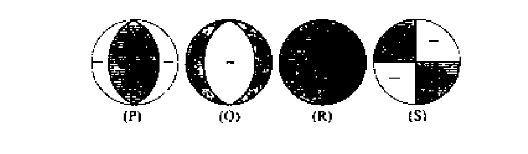
\includegraphics[width=0.5\linewidth]{figs/03.png} 
    \caption{}
    \label{fig:3}
\end{figure}
\begin{enumerate}
    \item P
    \item Q
    \item R
    \item S
\end{enumerate}
\end{multicols}

\item  The anelastic attenuation of seismic energy depends on

\hfill (GATE GG 2010) 

\begin{enumerate}
    \item  quality factor
\item  particle acceleration
\item stress drop
\item  particle velocity
\end{enumerate}
 \item The seismic wave travelling in low velocity layer and critically incident at the discontinuity between low and high velocity layers
 
 \hfill (GATE GG 2010) 
 
\begin{enumerate}
    \item  will be diffracted
\item  will be reflected
\item  will propagate along the discontinuity
\item will be absorbed
\end{enumerate}

\item An input signal $\cbrak{-1,1,0,2}$, after passing through a delay 
operator z,will be\\

\hfill (GATE GG 2010) 

\begin{enumerate}

    \item -z$^2$ $+$ z$^3$ $+$ $2$z$^5$
    \item $\cbrak{0,-1,1,0,2}$
    \item $\cbrak{0,2,0,1,-1}$
    \item -z$+$ z$^2$+$2$z$^4$
\end{enumerate}
\item If m represents the number of model parameters, d the number of data points and p the rank of matrix to be inverted, then which of the following defines an underdetermined system?
\hfill (GATE GG 2010) 
\begin{enumerate}
    \item  m $<$d and p$=$ d
\item  m$>$d and p$=$d
\item  m$=$d and p$=$d
\item  m$<$d and p$\neq$d
\end{enumerate}

\item A unit amplitude of an electromagnetic wave at thrice the skin-depth will be reduced to

\hfill (GATE GG 2010) 
\begin{multicols}{4}

\begin{enumerate}
    \item $-3$e
\item $\frac{3}{\text{e}}$
\item $\frac{\text{e}}{3}$
\item $e^{-3}$
\end{enumerate}
\end{multicols}

\item The Hilbert transform of a function $f\brak{t}$ is denoted by H\brak{f\brak{t}} . If $f\brak{t}$=$\sin{t}$, then H\cbrak{H\brak{f\brak{t}}}  is

\hfill (GATE GG 2010) 
\begin{multicols}{4}

\begin{enumerate}
    \item $-\sin{t}$
\item $-\cos{t}$
\item $\sin{t}$
\item $\cos{t}$
\end{enumerate}
\end{multicols}

\item The rectangular function $\pi$\brak{t} is defined as $\pi$\brak{t}= $1$ \hspace{0.7cm}   $\abs{t}\leq \frac{1}{2}$\\
\hspace*{6.7cm} $=0$ \hspace{0.7cm} $\abs{t} >\frac{1}{2}$\\
The convolution of $\pi$\brak{t} with itself will be 

\hfill (GATE GG 2010) 


\begin{enumerate}
    \item a triangular function $\triangle\brak{t}$
    \item  again $\pi$\brak{t}
\item a unit-step function u(t)
\item a delta function $\delta\brak{t}$
\end{enumerate}


\item Given A$=e^{-y}$\brak{\cos{x}{a_x}-\sin{x}{a_y}},where ${a_x}$ and $a_y$ denote the unit vectors in x-,y- directions respectively.Then $\nabla\cdot\brak{\nabla \times A}=$ 

\hfill(GATE GG 2010)
\begin{multicols}{4}
\begin{enumerate}
    \item $e^{-y}$
    \item 0
    \item $e^{-y}\cos{x}$
    \item $e^{-y}\sin{x}$
\end{enumerate}
\end{multicols}

\item Match the items in Group I with those in Group II.

\hfill (GATE GG 2010) \\
\begin{tabular}{ l l }
\textbf{Group I} & \textbf{Group Il}\\

P. convolution in time domain & 1. $\frac{1}{2\triangle t}$\\
Q. Nyquist frequency & 2. Flat spectrum\\
R. Aliasing & 3. Multiplication in frequency domain\\
S. White noise & 4. Frequency folding\\
& 5. Autocorrelation function
\end{tabular}

\begin{enumerate}
    \item P-$3$, Q-$1$, R-$4$, s-$2$
    \item P-$2$, Q-$1$, R-$5$, s-$4$
     \item P-$3$, Q-$1$, R-$2$, s-$1$
      \item P-$2$, Q-$4$, R-$1$, s-$5$
\end{enumerate}

\item In magnetic materials, the relation between magnetic permeability $\mu$ and susceptibility $K$ (in Sl units) is

\hfill (GATE GG 2010) 

\begin{enumerate}
    \item $\mu =1/k$
    \item $\mu 1-k$
    \item $\mu=1+k$
    \item $\mu=1-2\pi k$
\end{enumerate}
\vspace{0.7cm}
\textbf{Common Data Questions}\\
\vspace{0.6cm}
\textbf{Common Data Questions 48 and 49}\\
The terrain correction in gravity method accounts for topographic relief in the vicinity of the observation point. The Bouguer slab assumes the topography around the observation point to be flat. In the figure below, the Bouguer slab thickness is and the hollow portion P lies within the Bouguer slab. Q and R are parts of the topography.

\begin{figure}[H]
    \centering
    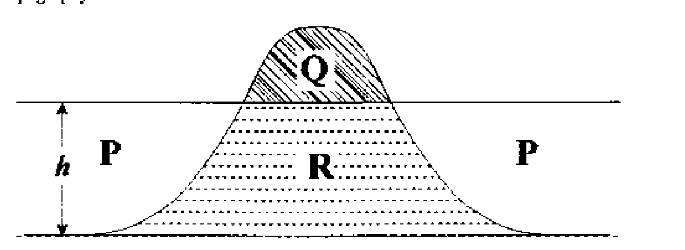
\includegraphics[width=0.5\linewidth]{figs/04.png} 
    \caption{}
    \label{fig:4}
\end{figure}
\item In the region P, the terrain correction is

\hfill (GATE GG 2010) 

\begin{enumerate}
    \item  half of that in R
    \item negative
\item  zero
\item positive 
\end{enumerate}
\item In the region Q, the terrain correction is required to account for

\hfill (GATE GG 2010) 

\begin{enumerate}
    \item  hollow portion P
\item  reduced gravity due to excess mass in portion Q
\item  increased gravity due to excess mass in portion Q
\item  over-correction of Bouguer slab

\end{enumerate}
\textbf{Common Data for Questions 50 and 51:}
For an input $x_n$ the output of a digital filter $y_n$ is given by $y_n$ $=1.5$$x_n$$-2$$x_{n-1}$$+     2.5$$y_{n-2}$
\item The order of the digital filter is

\hfill (GATE GG 2010) 
\begin{multicols}{4}

\begin{enumerate}
    \item  4
    \item 3
\item 2
\item 1 
\end{enumerate}
\end{multicols}

\item The transfer function of the digital filter is

\hfill (GATE GG 2010) 
\begin{multicols}{2}

\begin{enumerate}
    \item $\frac{y_n}{x_n}=\frac{1.5-2z}{1-2.5z}$
    \vspace{0.3cm}
    \item $\frac{y_n}{x_n}=\frac{1.5-2z}{1-2.5z^2}$
    \vspace{0.3cm}
    \item  $\frac{y_n}{x_n}=\frac{1-2.5z^2}{1.5-2z}$
    \vspace{0.3cm}
    \item $\frac{y_n}{x_n}=\frac{1.5-2z}{1+2.5z^2}$
\end{enumerate}
\end{multicols}

\vspace{0.3cm}
\textbf{Linked Answer Questions}
\textbf{Statement for Linked Answer Questions 52 and 53:}
In a two-layer earth model, the values of seismic velocity and density of first and second layers, respectively, are V$\rho 1$ $= 4000 \text{m/s}$.$\rho 1$ $=2500$kg/m$^3$,and  V$\rho 2$ $= 4500 \text{m/s}$.$\rho 2$ $=2600$kg/m$^3$.
\item The acoustic impedance of the first layer in SI units at normal incidence is

\hfill (GATE GG 2010) 
\begin{multicols}{4}

\begin{enumerate}
    \item  $10^3$
\item  $10^4$
\item  $10^5$
\item  $10^7$
\end{enumerate}
\end{multicols}

\item he transmission coefficient for a wave at normal incidence at the boundary of first and second layer is

\hfill (GATE GG 2010) 
\begin{multicols}{4}

\begin{enumerate}
    \item  0.46
\item 0.58
\item 0.92
\item  1.07
\end{enumerate}
\end{multicols}

\textbf{Statement for Linked Answer Questions 54 and 55:}

Consider a magnetotelluric \brak{MT} field set up. A plane electromagnetic wave with a time dependence factor $e^{(-i\omega t)}$ is travelling vertically downwards (z-direction) into the Earth with an angular frequency $\omega$ The electric field is polarized in the x-direction (strike).
\item The electromagnetic field components considered in this mode are

\hfill(GATE GG 2010)
\begin{multicols}{4}
\begin{enumerate}
    \item ${E_x,H_x,H_z}$
    \item ${E_z,H_x,H_z}$
    \item ${E_x,H_x,E_z}$
    \item ${E_z,H_x,H_z}$
\end{enumerate}
\end{multicols}

\item Which of the following equations represents the above mode?

\hfill (GATE GG 2010) 
\begin{multicols}{4}

\begin{enumerate}
    \item ${E_z=\frac{-1}{i\omega t}\frac{\partial{H_z}}{\partial z}}$
    \vspace{0.3cm}
    \item ${H_x=\frac{-1}{i\omega t}\frac{\partial{E_z}}{\partial z}}$
      \vspace{0.3cm}
    \item ${H_x=\frac{-1}{i\omega t}\frac{\partial{E_x}}{\partial z}}$
      \vspace{0.3cm}
    \item ${H_z=\frac{-1}{i\omega t}\frac{\partial{E_x}}{\partial z}}$\\
    \vspace{0.5cm}
    
\end{enumerate}
\end{multicols}
\textbf{END OF SECTION 2 OF PART B}
\vspace{3cm}

\textbf{General Aptitude (GA) Questions}
\item His rather casual remarks on politics his lack of seriousness about the subject.

\hfill (GATE GG 2010) 

\begin{enumerate}
    \item  masked
\item  belied
\item  betrayed
\item  suppressed
\end{enumerate}

\item Which of the following options is the closest in meaning to the word below:\\
\textbf{Circuitous}

\hfill (GATE GG 2010) 

\begin{enumerate}
    \item cyclic
\item  indirect
\item confusing
\item  crooked
\end{enumerate}

\item  If we manage to our children. our natural resources, we would leave a better planet for

\hfill (GATE GG 2010) 

\begin{enumerate}
    \item  uphold
\item  restrain
\item  cherish
\item  preserves
\end{enumerate}

\item $25$ persons are in a room. $15$ of them play hockey, $17$ of them play football and $10$ of them play both hockey and football. Then the number of persons playing neither hockey nor football is:

\hfill (GATE GG 2010) 
\begin{multicols}{4}

\begin{enumerate}
\item  $2$
\item  $17$
\item  $13$
\item  $3$
\end{enumerate}
\end{multicols}

\item The question below consists of a pair of related words followed by four pairs of words. Select the pair that best expresses the relation in the original pair.
\textbf{Unemployed: Worker}

\hfill (GATE GG 2010) 

\begin{enumerate}

    \item  fallow: land
\item  unaware: sleeper
\item  wit: jester
\item  renovated: house
\end{enumerate}

\item If $137 +276 = 435$ how much is $731 + 672$?

\hfill (GATE GG 2010) 
\begin{multicols}{4}

\begin{enumerate}
    \item  $534$
\item  $1403$
\item  $1623$
\item  $1513$
\end{enumerate}
\end{multicols}

\item  Hari \brak{H}, Gita \brak{G}, Irfan \brak{I} and Saira \brak{S} are siblings \brak{i.e. brothers and sisters}. All were born on $1^{st}$ January. The age difference between any two successive siblings (that is born one after another) is less than $3$ years. Given the following facts:

i. Hari's age$+$ Gita's age $>$ Irfan's age $+$ Saira's age.

ii. The age difference between Gita and Saira is I year. However, Gita is not the oldest and Saira is not the youngest.\\
iii. There are no twins\\
In what way they were born\brak{oldest first}?

\hfill (GATE GG 2010) 
\begin{multicols}{4}

\begin{enumerate}
    \item  HSIG
\item  SGHI
\item  IGSH
\item  IHSG

\end{enumerate}
\end{multicols}

\item \textbf{Modern warfare has changed from large scale clashes of armies to suppression of civilian populations. Chemical agents that do their work silently appear to be suited to such warfare; and regretfully, there exist people in military establishments who think that chemical agents are useful tools for their cause.}
Which of the following statements best sums up the meaning of the above passage:




\begin{enumerate}
    \item  Modern warfare has resulted in civil strife.

\item  Chemical agents are useful in modern warfare.
\item  Use of chemical agents in warfare would be undesirable.
\item  People in military establishments like to use chemical agents in war.
\end{enumerate}


\item  $5$ skilled workers can build a wall in $20$ days: $8$ semi-skilled workers can build a wall in $25$ days: $10$ unskilled workers can build a wall in $30$ days. If a team has $2$ skilled. $6$semi-skilled and $5$ unskilled workers, how long will it take to build the wall? 

\hfill(GATE GG 2010)

\begin{enumerate}
\begin{multicols}{4}
    \item $20$ days
    \item $18$ days
    \item $16$ days 
    \item $15$ days
\end{multicols}
\end{enumerate}

\item Given digits $2, 2, 3, 3, 3, 4, 4, 4, 4$ how many distinct $4$ digit numbers greater than $3000$ can be formed?

\hfill (GATE GG 2010) 
\begin{multicols}{4}

\begin{enumerate}
   
        \item $50$
        \item $51$
        \item $52$
        \item $53$
        
\end{enumerate}
\end{multicols}
\end{enumerate}
\textbf{END OF THE QUESTION PAPER}




\end{document}
